\chapter{図表の挿入}
\label{chp:chart}

\section{図の表示}
\label{sec:chart_figure}
    図を表示する場合,figure環境を使用します.画像はpng、jpg、pdfが使用できます.\\

    |記述例:PNG|
    \begin{verbatim}
    \begin{figure}[!h]
    \begin{screen}
    \begin{center}
        
\includegraphics[scale=0.4, clip]{./img/apple.png}    
        \caption{図の名前}
        \label{fig:図の名前}
    \end{center}
    \end{screen}
    \end{figure}
    \end{verbatim}

    |表示例:PNG|
    \begin{figure}[!h]
    \begin{screen}
    \begin{center}
        
\includegraphics[scale=0.4, clip]{./img/apple.png}
        \caption{図の名前}
        \label{fig:図の名前}
    \end{center}
    \end{screen}
    \end{figure}

    |記述例:JPG|
    \begin{verbatim}
    \begin{figure}[!h]
    \begin{screen}
    \begin{center}
        
\includegraphics[scale=0.4, clip]{./img/CIT.jpg}    
        \caption{図の名前}
        \label{fig:図の名前}
    \end{center}
    \end{screen}
    \end{figure}
    \end{verbatim}

    |表示例:|
    \begin{figure}[!h]
    \begin{screen}
    \begin{center}
        
\includegraphics[scale=0.4, clip]{./img/CIT.jpg}
        \caption{図の名前}
        \label{fig:図の名前}
    \end{center}
    \end{screen}
    \end{figure}

    |記述例:PDF|
    \begin{verbatim}
    \begin{figure}[!h]
    \begin{screen}
    \begin{center}
        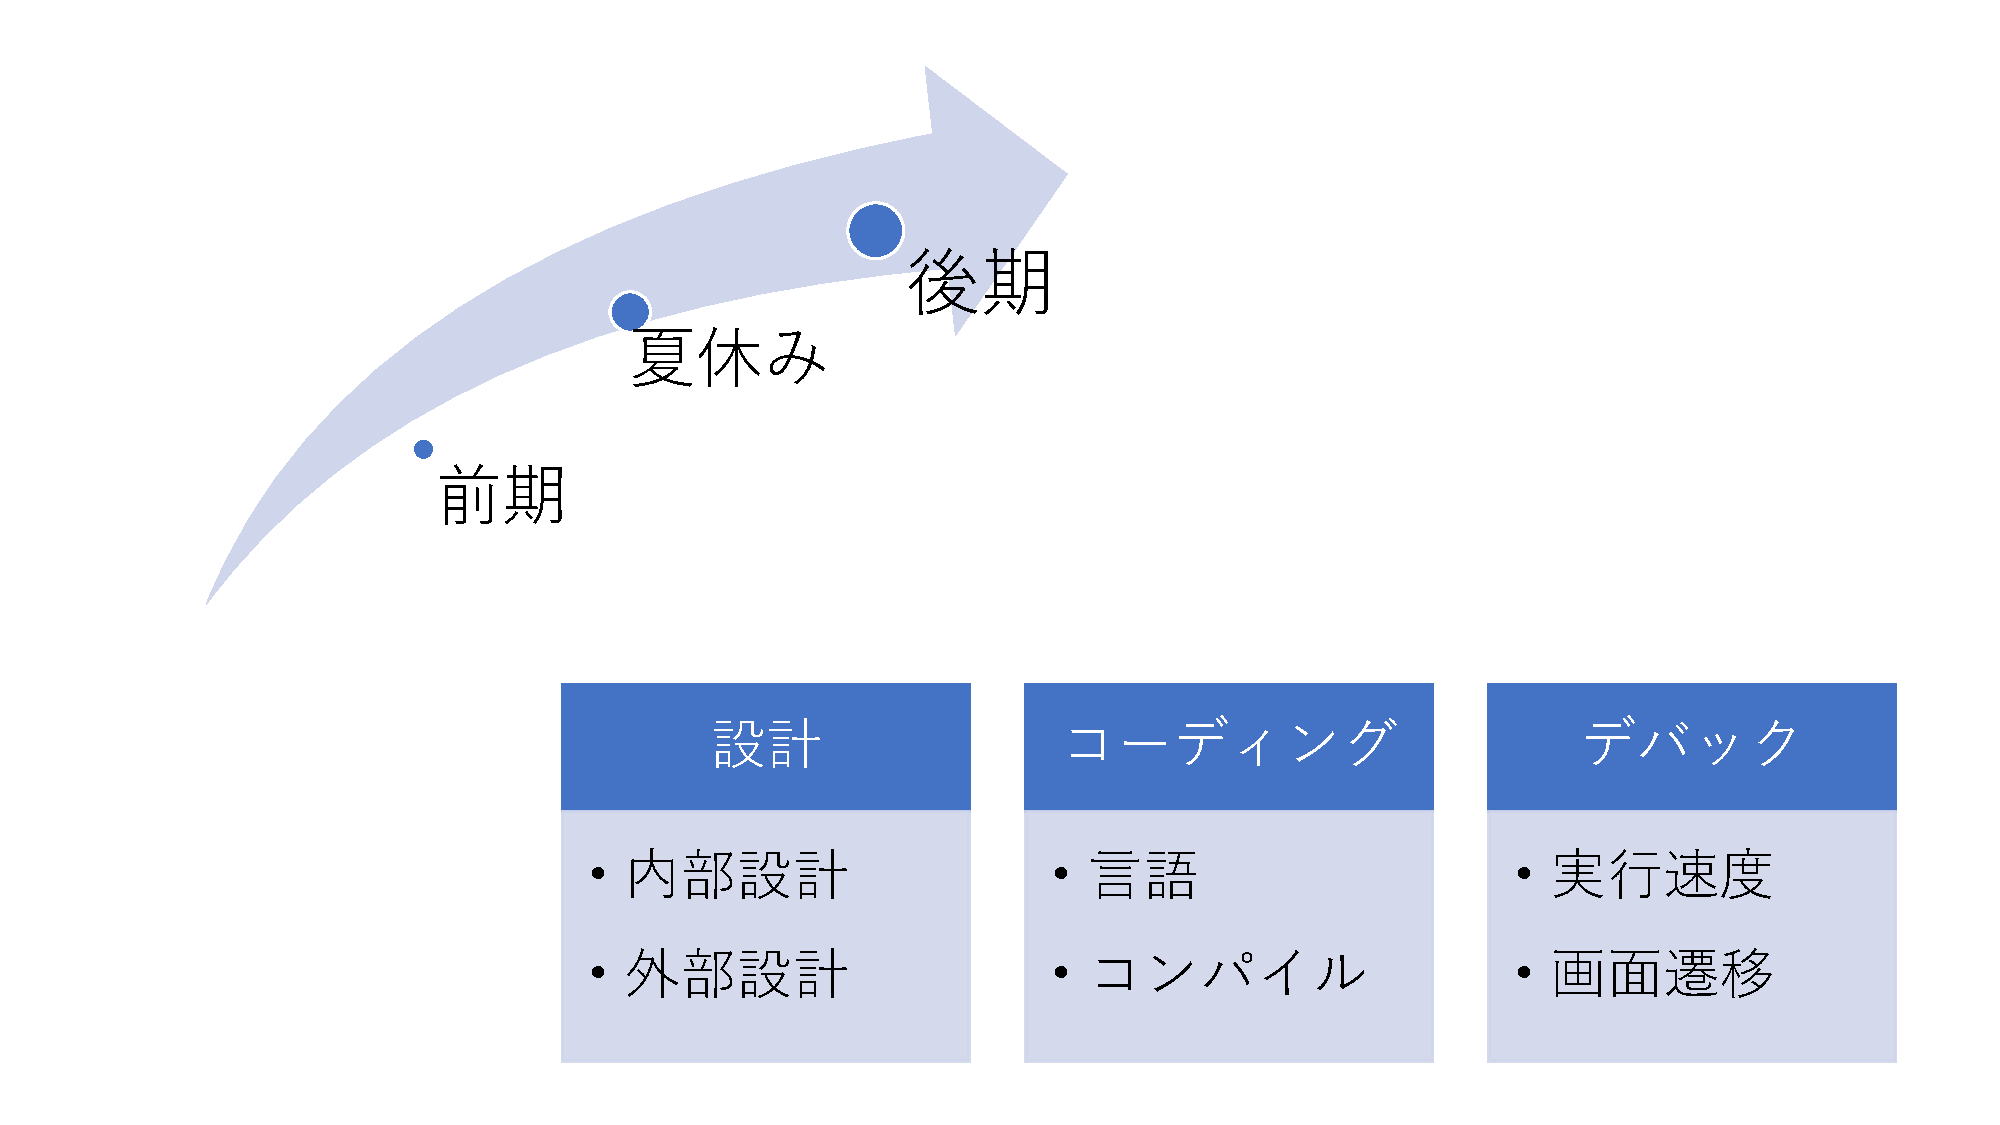
\includegraphics[scale=0.4, clip]{./img/illust.pdf}    
        \caption{図の名前}
        \label{fig:図の名前}
    \end{center}
    \end{screen}
    \end{figure}
    \end{verbatim}

    |表示例:PDF|
    \begin{figure}[!h]
    \begin{screen}
    \begin{center}
        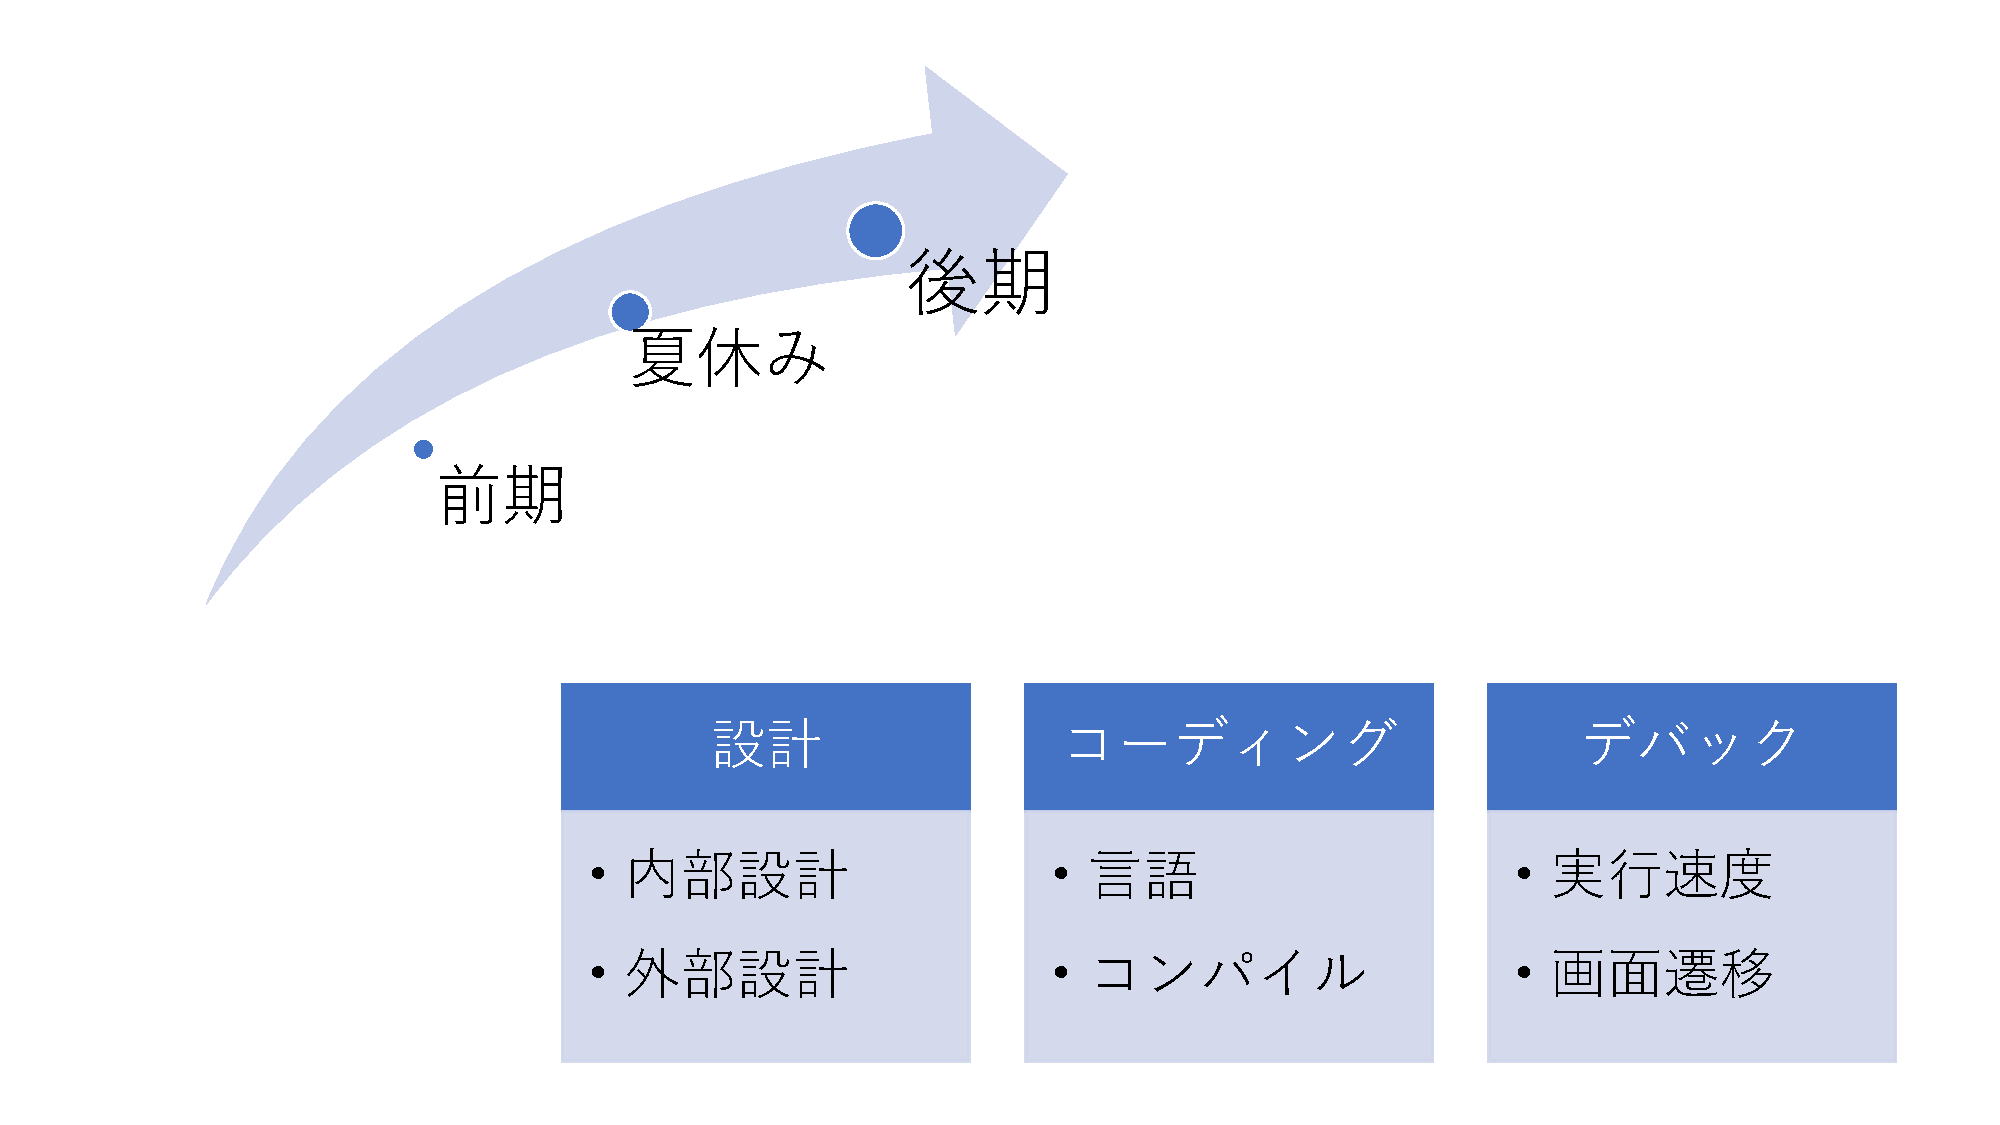
\includegraphics[scale=0.4, clip]{./img/illust.pdf}
        \caption{図の名前}
        \label{fig:図の名前}
    \end{center}
    \end{screen}
    \end{figure}


    \begin{itemize}
        \item figure環境

        図を表示するための場所を作ります.[!h]は「なるべくその場所に表示する」というオプションです.
        \item screen環境

        図を囲むための枠を表示します.
        \item center環境

        囲んだ部分を中央ぞろえで表示します.
        \item includegraphicsコマンド

        図を表示します.\{\}内に表示する図のパスを記述します.[scale=0.4, clip]は「拡大率0.4ではみ出した部分は切り取る」というオプションです.\\
        オプションには「width」「height」「angle」があります.カンマで区切ることで複数指定することが可能です.
	 \item captionコマンド
	
	 図にキャプションをつけます。番号は自動で振られます。
    \end{itemize}
    labelコマンドについては\ref{sec:reference_chapter}を参照してください.

\section{表の表示}
\label{sec:chart_table}
    表を表示する場合,table環境を使用します.一行は\&で区切ります.行端には改行を記述します.\\
    |記述例|
    \begin{verbatim}
    \begin{table}[!h]
    \begin{center}
    \caption{表の名前}
    \label{fig:表の名前}
    \begin{tabular}{|l|c|r||r|}
    \hline
        \multicolumn{2}{|l|}{メニュー} 
            & \multicolumn{1}{c||}{値段} 
                & \multicolumn{1}{p{8\zw}|}{カロリー}\\ \hline \hline
             & 並盛 & 500円 & 600 kcal \\ \cline{2-4}
        牛丼 & 大盛 & 1,000円 & 800 kcal \\ \cline{2-4}
             & 特盛 & 1,500円 & 1,000 kcal \\ \hline
             & 並盛 & 300円 & 250 kcal \\ \cline{2-4}
        牛皿 & 大盛 & 700円 & 300 kcal \\ \cline{2-4}
             & 特盛 & 1,000円 & 350 kcal \\ \hline
    \end{tabular}
    \end{center}
    \end{table}
    \end{verbatim}

|表示例|
		\newcolumntype{Y}{>{\centering\arraybackslash}p{10\zw}}
    \begin{table}[!h]
    \begin{center}
    \caption{表の名前}
    \label{fig:表の名前}
    \begin{tabular}{|l|c|r||r|}
    \hline
            \multicolumn{2}{|Y|}{メニュー} & \multicolumn{1}{c||}{値段} & \multicolumn{1}{p{8\zw}|}{カロリー}\\ \hline \hline
             & 並盛 & 500円 & 600 kcal \\ \cline{2-4}
            牛丼 & 大盛 & 1,000円 & 800 kcal \\ \cline{2-4}
             & 特盛 & 1,500円 & 1,000 kcal \\ \hline
             & 並盛 & 300円 & 250 kcal \\ \cline{2-4}
            牛皿 & 大盛 & 700円 & 300 kcal \\ \cline{2-4}
             & 特盛 & 1,000円 & 350 kcal \\ \hline
    \end{tabular}
    \end{center}
    \end{table}
    \begin{itemize}
    \item table環境

    表を表示するための場所を作ります.
       \item tabular環境

       表を表示します.\{\}内に列の書式を設定しています.\\
    l:左寄せ c:センタリング r:右寄せ |:縦罫線\\
    表内に文章を入れる場合や,カラム幅を指定したい場合は列書式に「\verb|p{5cm}|」のように記述します.カラム幅を指定しない場合は自動で幅が設定されます.
    \item hlineコマンド

    横罫線を表示します.
    \item clineコマンド

    特殊横罫線を表示します.\{\}内に線を引きたいカラムを指定します.上記では2~4カラムを指定しています.
    \item multicolumnコマンド

    カラムを結合します.\verb|\multicolumn{結合カラム数}{書式}{文字列}|
    \end{itemize}

